\scanpage{36}
\noindent\makebox[0pt][r]{(40)\quad}\(\left\{\begin{minipage}{.44\linewidth}\raggedright\footnotesize
$\deleted{\unsure{\underline\omega_\Delta}}C_\Delta$ (\textquotedblleft \unsure{colors|colours|couleurs}\textquotedblright)
\par ens. des $2$ tétraèdres (échangés par l'antipodisme) inscrits dans le cube qui correspond à $\Delta$

\figure{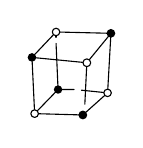
\begin{tikzpicture}[scale=.85,line cap=round,line join=round]
\draw (0,.84)--(.82,.76)--(1.18,1.20)--(.36,1.22)--cycle;
\draw (0,.84)--(.04,0)--(.39,.36)--(.36,1.05);
\draw (.36,1.14)--(.36,1.22);
\draw (.04,0)--(.76,-.02)--(1.13,.31)--(1.18,1.20);
\draw (.82,.76)--(.79,.14);
\draw (.39,.36)--(.63,.36) (.74,.35)--(1.13,.31);
\fill (0,.84) circle (.064) (1.18,1.20) circle (.065) (.76,-.02) circle (.066) (.39,.36) circle (.063);
\draw[fill=white] (.36,1.22) circle (.056) (.82,.76) circle (.058) (.04,0) circle (.057) (1.13,.31) circle (.056);
\end{tikzpicture}}

ou encore des deux couleurs (échangés\ldots) des faces de l'octaèdre $\Delta$

\figure{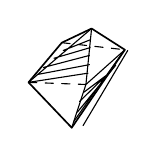
\begin{tikzpicture}[scale=.9,line cap=round,line join=round]
\draw[line width=.6pt] (0,.56)--(.47,1.12)--(.89,1.32)--(1.36,1.02)--(.61,-.08)--cycle;
\draw (.89,1.32)--(.81,.53)--(.61,-.08) (.81,.53)--(1.36,1.02);
\draw[dashed] (0,.56)--(.81,.53) (.47,1.12)--(1.36,1.02);
\draw (0,.56)--(.89,1.32) (0,.56)--(.84,.69) (.12,.67)--(.86,.81)
(.21,.77)--(.86,.94) (.36,.90)--(.87,1.05) (.49,1.01)--(.87,1.16);
\draw (.64,.01)--(1.32,.97) (.69,.14)--(1.23,.80) (.72,.29)--(1.17,.73)
(.78,.42)--(1.10,.66) (1.40,1.01)--(.77,-.05);
\end{tikzpicture}}

correspond au car. \deleted{\unsure{mixte}} de $\mathrm{Aut}_{\mathrm{oct}}^+(\Delta)\times\{1,\underline a_\Delta\}$

\uline{NB} On a $F(\Delta)\simeq\underline C_\Delta\times\underline I_\Delta$ où $I_\Delta=F(\Delta)/\underline a_\Delta$ est l'ens. des quatre directions de faces

\end{minipage}\quad\begin{minipage}{.22\linewidth}\raggedright\footnotesize
$\mathrm{or}(\Delta)$

ens des deux orientations de l'octaèdre $\Delta$

$\simeq$

correspond au car. non trivial de $\{1,\underline a_\Delta\}$

\end{minipage}\quad\begin{minipage}{.22\linewidth}\raggedright\footnotesize
$\deleted{\unsure{C_\Delta\wedge\mathrm{or}(\Delta)}}$
$\underline\omega_\Delta=\underline\omega_{I_\Delta}$

ens. des deux orientations de $I_\Delta$, ou encore, de $J_\Delta$

correspond au caractère non-trivial de $\mathrm{Aut}_{\mathrm{oct}}^+(\Delta)$
\end{minipage}\right.\)

qui satisfont à un iso. canonique

\[
\deleted{\unsure{C_\Delta\wedge}}\mathrm{or}(\Delta)\wedge\underset{\llcorner\mkern-2mu\rule{.85em}{.35pt}\mkern-2mu\lrcorner}{\underline\omega_\Delta}\wedge\underline C_\Delta
\simeq\mathbb 1_{\mathbb F_2}. \tag*{(41)}
\]

On a un isom.

\[
\left\{\begin{aligned}
 C_\Delta&=\bigwedge_{i\in J}\Delta_i\quad\text{quotient de }
 \overbrace{\prod_{i\in J}\Delta_i=F(\Delta)}^{\text{torseur sous }\mathbb F_2^J}\\
 &\text{pour }\underset{\substack{\rotatebox[origin=c]{90}{$\scriptstyle\simeq$}\\\underbrace{V_J(\mathbb F_2)}_{M_0}\times\mathbb F_2}}{\mathbb F_2^J}
 \xrightarrow{\underbrace{(\text{somme})}}\mathbb F_2\\
 \text{i.e.}\quad C_\Delta&=\underbrace{F(\Delta)/M_0}_{} 
\end{aligned}\right. \tag*{(42)}
\]

($P_M/(M_0\times\unsure{\mathfrak z})\deleted{\unsure{\times M_0}}$ dans le cas qui nous occupe) correspond au car. $\mathrm{sg}(g).\det(g)$ dans le cas \deleted{\unsure{qui}} où $\Delta$ est défini par un $M$)

\reversemarginpar\margin{donc dans ce cas on a $C_\Delta\simeq\mu\wedge\underline\omega$}\normalmarginpar

\[
 \underline\omega_\Delta=\underline\omega_{I_\Delta}=\underline\omega_J
 \quad\text{l'ens à deux éléments associé à }J
 \tag*{\deleted{\unsure{(42)}}(43)}
\]

(correspond au caractère $\mathrm{sg}(g)$ dans le cas d'un $M$)

\[
 \deleted{\unsure{\underline\omega}}\mathrm{or}(\Delta)\simeq
 \underset{\underline\omega_J}{\underline{\underline\omega_\Delta}}\wedge C_\Delta \tag*{(44)}
\]

(correspond au caractère $\det(g)$ dans le cas d'un $M$) \unsure{d'où|donc} $\left\lfloor\underline{\mathrm{or}(\Delta)\simeq\mu\overset{\mathrm{def}}{=}(\det M)^*}\right\rfloor$.

L'octaèdre \uline{orienté} \inserted{$\Delta^+$} associé à $M$ est défini par le torseur $P_M/\mathbb F_2^{\underline\omega}$ sous $M_0=V_J(\mathbb F_2)$, i.e. par
% archive sheet number: 35
